\chapter{AWS Deployment \\
\small{\textit{-- Ivan Farfan, Johan Jaramillo, Ryan Davis}}}
\index{AWSDeployment} 
\index{Chapter!AWSDeployment}
\label{Chapter::AWSDeployment}

\section{Deployment Steps \& Commands (Local \texorpdfstring{$\rightarrow$}{->} AWS)}
This section summarizes the steps I used to containerize the two-buttons site locally and deploy it to AWS.
The flow follows our prior Docker and AWS notes. :contentReference[oaicite:0]{index=0}

\subsection{Local Build \& Run (Docker)}
\begin{minted}{bash}
# From the app directory containing Dockerfile (Express + /public)
docker build -t color-buttons-app .
docker run -p 8080:3000 color-buttons-app
# Visit http://localhost:8080
\end{minted}

\subsection{Authenticate \& Push to ECR}
\begin{minted}{bash}
# (Set once per shell; edit to your values)
export AWS_REGION=us-east-1
export ECR_REPO=color-buttons-app
export IMAGE_TAG=v1
export AWS_ACCOUNT_ID="$(aws sts get-caller-identity --query Account --output text)"

# Create (idempotent) repo if not present
aws ecr describe-repositories \
  --repository-names "$ECR_REPO" \
  --region "$AWS_REGION" >/dev/null 2>&1 || \
aws ecr create-repository \
  --repository-name "$ECR_REPO" \
  --image-scanning-configuration scanOnPush=true \
  --region "$AWS_REGION"

# Login Docker to ECR
aws ecr get-login-password --region "$AWS_REGION" \
| docker login --username AWS --password-stdin \
  "$AWS_ACCOUNT_ID.dkr.ecr.$AWS_REGION.amazonaws.com"

# Build for common runtime (x86) if on Apple Silicon
docker build --platform linux/amd64 -t "$ECR_REPO:$IMAGE_TAG" .

# Tag \& push to ECR
docker tag "$ECR_REPO:$IMAGE_TAG" \
  "$AWS_ACCOUNT_ID.dkr.ecr.$AWS_REGION.amazonaws.com/$ECR_REPO:$IMAGE_TAG"

docker push "$AWS_ACCOUNT_ID.dkr.ecr.$AWS_REGION.amazonaws.com/$ECR_REPO:$IMAGE_TAG"
\end{minted}

\subsection{Quick Deploy with AWS App Runner}
\begin{minted}{bash}
export APP_NAME=color-buttons-apprunner
export CONTAINER_PORT=3000

aws apprunner create-service \
  --service-name "$APP_NAME" \
  --region "$AWS_REGION" \
  --source-configuration "{
    \"ImageRepository\": {
      \"ImageIdentifier\": \"$AWS_ACCOUNT_ID.dkr.ecr.$AWS_REGION.amazonaws.com/$ECR_REPO:$IMAGE_TAG\",
      \"ImageRepositoryType\": \"ECR\",
      \"ImageConfiguration\": {\"Port\": \"$CONTAINER_PORT\"}
    },
    \"AutoDeploymentsEnabled\": true
  }" \
  --instance-configuration "{\"Cpu\":\"1 vCPU\",\"Memory\":\"2 GB\"}"
\end{minted}

\noindent After creation, obtain the public URL:
\begin{minted}{bash}
aws apprunner list-services \
  --region "$AWS_REGION" \
  --query "ServiceSummaryList[?ServiceName=='$APP_NAME'].ServiceUrl" \
  --output text
\end{minted}

\subsection{Live Links}

\noindent \textbf{AWS App Runner URL:}\\
\href{https://6ibmrtgk5s.us-east-2.awsapprunner.com/}{\texttt{https://6ibmrtgk5s.us-east-2.awsapprunner.com/}}


\section{Updated Design Class Diagram}
\begin{figure}[h]
  \centering
  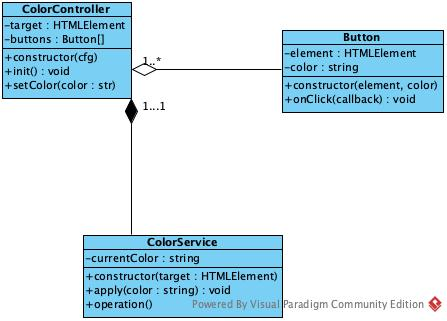
\includegraphics[width=0.7\textwidth]{png/colorButtonPage.jpg}
  \caption{UML Class Diagram for the Refactored Website}
  \label{fig:colorPageClassDiagram}
\end{figure}

